% ============================================================
% Chapter 2 – Related work
% chapters/02-related-work.tex
% ============================================================

\chapter{Related work}
\label{chap:related-work}

This chapter introduces the background and the state of the art.


\section{Background}

\subsection{Knowledge Graphs}

A knowledge graph (KG) is a structured representation of knowledge that captures entities, their attributes, and the relationships between them as a directed graph. Nodes in a knowledge graph represent entities, which can be anything from people and places to concepts and events, while edges between those nodes are labelled to indicate the type of relationship that holds between the entities.

\begin{figure}[htbp]
\centering
\begin{minipage}{0.6\textwidth}
    \centering
    %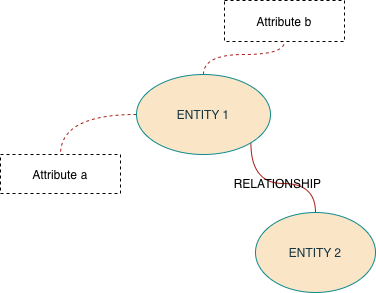
\includegraphics[width=0.8\textwidth]{img/KG-example.png}
    \includesvg[width=0.8\textwidth]{img/KG-example.svg}
\end{minipage}
\hfill
\begin{minipage}{0.35\textwidth}    
    \caption{An example of a structure of a knowledge graph containing two entities related with each other, the first one with two attributes.}
\end{minipage}
\label{fig:kg-example}
\end{figure}

This graph-based representation makes connections between pieces of information explicit in a way that is both human-readable\footnote{The human-readability of a knowledge graph depends on its size and serialization format. Large graphs are typically explored via dedicated query languages such as SPARQL rather than read directly.} and machine-processable. % c'est pas tjrs human readble en fontion de la forme. voir l'exemple à la section suivante.

As a result, knowledge graphs are a powerful tool for applications such as search engines and data integration. % 

Various format can be used to represent a knowlege graph. The graphical representation is the most intuitive. For machine processing, this thesis focuses on RDF, which is a widely adopted standard representation. 

\subsection{RDF}

RDF, or Resource Description Framework, is a standard model defined by the World Wide Web Consortium (W3C) for representing information about resources on the Web. RDF provides a framework for expressing knowledge in the form of a graph built from three-part statements, known as triples. Each triple consists of:
\begin{itemize}
  \item a subject: the resource being described,
  \item a predicate: the property or relationship of that resource,
  \item an object: the value of the property, or another resource.
\end{itemize}

By combining many triples, RDF can represent complex graphs of interconnected resources. RDF also supports the integration of data from diverse sources and enables reasoning over these data, which makes it a fundamental technology for building and managing knowledge graphs.

Figure \ref{fig:rdf-example} illustrates a simple graph with its graphical representation, its RDF graphical represnation, its RDF triples and its TURTLE code. TURTLE is a popular RDF serialization format that provides a compact and human-readable syntax for expressing RDF triples. It uses prefixes to abbreviate URIs and allows for a more concise representation of RDF data compared to other formats like RDF/XML.
%TODO: Décrire en faite le graphe.


% Petit exemple concret de triple (en Turtle)
% et la représentation graphique correspondante, pour illustrer le lien entre RDF et KG.

\begin{figure}[htbp]
\centering
 \begin{minipage}{1.1\textwidth}
    \raggerleft
% --- (a) Graphe RDF avec IRIs ---
\begin{subfigure}[b]{0.45\textwidth}
\centering
\begin{tikzpicture}[
  node distance=0.9cm,
  uri/.style={draw=blue!50!green, ellipse, fill=orange!15,
              minimum width=1.8cm, minimum height=1.35cm,
              font=\footnotesize},
  lit/.style={draw=black!, rectangle, fill=blue!10,
              minimum width=1.7cm, minimum height=0.6cm,
              font=\footnotesize},
  ->, >=Stealth, draw=red!70!black, font=\footnotesize
]
  \node[uri] (student) {\texttt{students:s1}};
  \node[uri, below=1.1cm of student] (course) {\texttt{courses:c1}};
  \node[lit, above left=1.2cm and 0.1cm of student]
       (fname)  {\texttt{"Peter"\^{}\^{}xsd:string}};
  \node[lit, above right=1.2cm and 0.1cm of student]
       (year)   {\texttt{1\^{}\^{}xsd:integer}};
  \node[lit, below=0.9cm of course]
       (cname)  {\texttt{"Databases"\^{}\^{}xsd:string}};

  \draw (student) -- node[above]{\footnotesize\texttt{uni:enrolledIn}} (course);
  \draw (student) -- node[left] {\footnotesize\texttt{uni:firstName}}  (fname);
  \draw (student) -- node[right]{\footnotesize\texttt{uni:year}}       (year);
  \draw (course)  -- node[above]{\footnotesize\texttt{uni:courseName}} (cname);
\end{tikzpicture}
\caption{RDF graph with IRIs}
\label{fig:rdf-b}
\end{subfigure}
\hfill
% --- (b) Turtle ---
\begin{subfigure}[b]{0.5\textwidth}
\centering
\begin{lstlisting}[style=turtle]
@prefix uni:     <http://www.example.org/university#> .
@prefix students:<http://www.example.org/students#> .
@prefix courses: <http://www.example.org/courses#> .
@prefix xsd:     <http://www.w3.org/2001/XMLSchema#> .

students:s1
  a             uni:Student ;
  uni:firstName "Peter"^^xsd:string ;
  uni:year      1^^xsd:integer ;
  uni:enrolledIn courses:c1 .

courses:c1
  a              uni:Course ;
  uni:courseName "Databases"^^xsd:string .
\end{lstlisting}
\caption{Turtle serialisation}
\label{fig:rdf-d}
\end{subfigure}
\vspace{0.6em}
\end{minipage}

% --- (c) Triples ---

\begin{minipage}{0.4\textwidth}
    \raggerleft
\begin{subfigure}[b]{0.4\textwidth}
\centering
\footnotesize
\begin{tabular}{@{}lll@{}}
\toprule
\textbf{Subject} & \textbf{Predicate} & \textbf{Object} \\
\midrule
\texttt{students:s1} & \texttt{rdf:type}        & \texttt{uni:Student} \\
\texttt{students:s1} & \texttt{uni:firstName}   & \texttt{"Peter"} \\
\texttt{students:s1} & \texttt{uni:year}        & \texttt{1} \\
\texttt{students:s1} & \texttt{uni:enrolledIn}  & \texttt{courses:c1} \\
\texttt{courses:c1}  & \texttt{rdf:type}        & \texttt{uni:Course} \\
\texttt{courses:c1}  & \texttt{uni:courseName}  & \texttt{"Databases"} \\
\bottomrule
\end{tabular}
\caption{RDF triples}
\label{fig:rdf-c}

\end{subfigure}

\end{minipage}
\hfill
\begin{minipage}{0.55\textwidth}    
    \caption{%
      A university knowledge graph fragment, shown as
      (a)~an RDF graph with typed IRIs and literals,
      (b)~the corresponding list of triples, and
      (c)~the Turtle serialisation.
      This example is used as a running thread through
      Sections~\ref{sec:background-shacl} and~\ref{sec:background-rml}.
    }
\end{minipage}

\label{fig:rdf-example}

\end{figure}

% Description du graph exemple:
The graph models a student~\texttt{students:s1} (Peter, year~1) enrolled in a course~\texttt{courses:c1} (Databases). Figure~\ref{fig:rdf-b} reveals a structural property of RDF that is central to this thesis: \emph{a single resource can simultaneously be the object of one triple and the subject of others.}
Here, \texttt{courses:c1} is the object of the \texttt{uni:enrolledIn} triple originating from \texttt{students:s1}, yet it is also the subject of its own \texttt{uni:courseName} triple. Multiple students in the full dataset share the same
course nodes: for instance, \texttt{students:s1}, \texttt{s2}, and~\texttt{s9} all point to~\texttt{courses:c1}. This \emph{shared-node}
topology — which distinguishes RDF graphs from trees — is exactly what makes form-based RDF authoring non-trivial: a form generator cannot simply traverse the shape hierarchy top-down, because the same node may need to be reused across multiple branches of the form. We return to this problem in Chapter~\ref{chap:conceptualisation}.

This university knowledge graph is drawn from a practical lab exercise on knowledge-graph construction, and serves as the running example for the SHACL and RML illustrations that follow.

\subsection{RML}
\label{sec:background-rml}

The RDF Mapping Language (RML) is a language designed to map heterogeneous data sources to RDF datasets. It allows one to define how a specific set of data should be transformed into RDF triples, mapping a variety of data formats (e.g., CSV, JSON, XML) into a graph-based format, namely RDF.

RML extends and broadens the capabilities of R2RML, the W3C recommendation for mapping relational databases to RDF, by supporting a wider range of data formats. While R2RML focused on relational databases, RML provides a more general language that can handle different kinds of data structures. It enables the expression of more complex mapping scenarios, including nested structures and relationships, making it a valuable tool for transforming and integrating data into RDF for use in knowledge graphs.

% TODO: add example here. P-e utliser le meme KG que la section préc.

Importantly, an RML mapping itself is represented as an RDF graph. This means that, beyond the complexity of the source data, the mapping definition also has a graph structure, which can be intricate and difficult to manipulate directly, especially for non-expert users. In this thesis, we leverage this specific characteristic of RML as a use case for exploring visual support for complex RDF graphs.

% TODO : introduire ici les limitations de RML-core qui nous intéressent
% (complexité des structures imbriquées, difficulté d'édition manuelle, etc.)
% et justifier brièvement le choix de RML-core comme cas d'étude.


\subsubsection{Tools related to RML}

Several tools have been developed to simplify the creation of RML mappings. For instance, RMLMapper and YARRRML provide higher-level syntaxes or utilities to help users describe mappings. However, these solutions are still primarily programming-oriented and require users to be comfortable with textual configuration files or domain-specific languages.

In the context of this thesis, we are interested in exploring the possibility of using a visual and generic (no-code) form-based approach to handle the complexity of RML mappings, and more generally RDF graphs. This is why we focus on forms generated from SHACL shapes rather than on existing textual mapping tools.

% TODO : comme j'ai testé en utilissant RMLMapper/YARRRML dans mon workflow,
% ajouter une phrase ou deux sur mon expérience (ce qui est pratique, ce qui reste difficile).

\subsection{SHACL}
\label{sec:background-shacl}

SHACL, or Shapes Constraint Language, is a W3C standard designed to validate RDF graphs against a set of conditions defined in the form of shapes. A shape is a collection of constraints that specifies the expected structure and properties of RDF data. 

\% À completer..

Constraints can include datatype restrictions, cardinality bounds, value ranges, or references to other node shapes, among others.

Because SHACL shapes are themselves RDF graphs, they can also be used as a high-level, machine-readable description of the structure of data that an application expects. This dual role—validation and structural description—makes SHACL particularly interesting for generating forms: the same shapes that constrain the data can be used as a specification for form fields, their types, and some aspects of their layout.

Another advantage of this dual role is that SHACL shapes can be treated like any other RDF graph. They can be written and stored in standard RDF serialisations such as Turtle or JSON-LD. This makes it possible to manage shape graphs with the same tooling and practices that are already used for data graphs.

% TODO : ajouter ici un petit exemple de shape simple (node shape + property shape),
% puis, plus tard, faire le lien avec les outils de génération de formulaires étudiés.


\section{Related work}

This section first introduces established SHACL-based form systems that have shaped how constraints can drive user interfaces. It then focuses on generic SHACL-based web form builders that most closely match the type of system we aim to develop for RML-core mappings.

\subsection{Foundational SHACL-based form systems}

\subsubsection{TopQuadrant, DASH, and TopBraid EDG}

TopQuadrant's work on form generation from SHACL provides an important foundation for understanding how constraints can drive user interfaces. The document ``Form Generation using SHACL and DASH'' shows how SHACL Core properties such as \texttt{sh:datatype} and \texttt{sh:maxCount}, originally designed for validation, can also be used to configure input widgets and validation rules in user input forms. It further explains how layout-oriented properties like \texttt{sh:order} and \texttt{sh:group} can be leveraged to structure form layouts into sections and to control the order of fields, for example grouping address-related properties in one section and contact information in another.\cite{dash-forms}

Beyond SHACL Core, the DASH (Data Shapes) vocabulary extends SHACL with additional terms that are particularly useful for form building, such as editor and viewer hints, default views, and suggestions.\cite{dash-spec} These DASH terms are used in TopBraid EDG, TopQuadrant's commercial knowledge graph platform, to define ``view shapes'' that not only constrain data but also specify how instances should be presented and edited in forms.\cite{topbraid-edg} In EDG, data entry forms are thus fully SHACL- and DASH-driven: the same shapes control both data validity and user interface behaviour.

In this thesis, DASH and TopBraid EDG serve primarily as conceptual and industrial references. They illustrate what advanced SHACL-driven UI generation can look like in a mature, enterprise-grade environment, but they are not considered as direct implementation candidates, because our goal is to start from lightweight, generic web form builders rather than from a proprietary platform.

% TODO: ajouter 1–2 exemples concrets tirés du document DASH
% (par ex. un cas où sh:group/sh:order sont utilisés, ou un exemple d'usage de dash:editor/dash:viewer)
% et les commenter brièvement.

\subsubsection{SHAPEness Metadata Editor (EPOS-EU)}

SHAPEness is a Java desktop application conceived to help users create and update RDF metadata descriptions.\cite{shapeness-github} It is a SHACL-driven multi-view editor: users work with different coordinated views to assess and improve the quality of metadata represented as RDF graphs, while SHACL shapes define the constraints that these metadata must satisfy. The tool has been developed and tested in the framework of the European Plate Observing System (EPOS), where it has proven useful to create and maintain valid graphs according to the EPOS data model and EPOS-DCAT-AP profiles.\cite{shapeness-paper}\cite{shapeness-knmi}

From the perspective of this thesis, SHAPEness demonstrates that rich SHACL-based editors are feasible and valuable in real scientific data ecosystems. It shows that SHACL can be used not only for batch validation but also as a backbone for interactive, multi-view editing workflows. However, SHAPEness is strongly oriented towards desktop usage and domain-specific metadata management, whereas our objective is to design a generic web-based form-builder for highly nested RML-core mapping structures.

% TODO: installer/exécuter SHAPEness ou à voir une démo,
% ajouter ici 2–3 phrases sur l'interface (types de vues, navigation dans le graphe, ressenti).

\subsection{SHACL-based web form builders}

In the remainder of this section, we focus on generic SHACL-based web form builders, as these tools are the closest to the type of system we aim to develop for RML-core mappings.

\subsubsection{ULB-Darmstadt/shacl-form}

ULB-Darmstadt/shacl-form is an HTML5 web component that generates and handles forms based on SHACL shapes. The core idea is to provide a reusable custom element, \texttt{<shacl-form>}, that takes a shapes graph as input and produces a form for creating or editing RDF data that conform to these shapes.\cite{ulb-darmstadt-shacl-form-demo} Shapes can be passed directly as Turtle strings via the \texttt{data-shapes} attribute, or loaded from a URL via \texttt{data-shapes-url}. Optional \texttt{data-values} and \texttt{data-values-url} attributes allow pre-populating the form from an existing data graph, and an event-based API exposes validation results and serialized RDF triples back to the application.\cite{ulb-darmstadt-shacl-form}\cite{ulb-darmstadt-npm}

The library maps SHACL datatypes and numeric constraints to corresponding HTML input elements and validation attributes, and it honours layout-related properties such as \texttt{sh:order} and \texttt{sh:group} to influence the order and grouping of fields. More advanced features include support for \texttt{sh:or}, where alternatives between node shapes can be presented in the UI, and options to collapse groups of fields to reduce visual complexity in larger forms. These aspects make ULB-Darmstadt/shacl-form a strong candidate for a standards-oriented form generation pipeline closely aligned with SHACL.

For RML-core, the main challenges relate to how the component behaves in the presence of deep nesting and complex constraint patterns. Highly nested node shapes corresponding to RML-core structures (e.g., logical sources and targets, join conditions, term maps) may require several levels of nested sections, which raises usability questions for authors working on large mappings.

% TODO: décrire ce que j'ai observé en testant des shapes inspirées de RML-core :
% - comment l'UI se comporte avec 2–3 niveaux d'imbrication (node shapes imbriqués),
% - ce que j'ai vu pour sh:or, sh:in,
% - si la navigation devient difficile ou reste gérable.

\subsubsection{hypermedia-app/Shaperone}

Shaperone is a web library dedicated to SHACL-driven form user interfaces, developed within the hypermedia-app ecosystem.\cite{shaperone-github} It exposes form UI elements that are driven by SHACL shapes and is organised around configurable ``component sets'', i.e., collections of UI widgets that can be plugged in to render different property types and shapes.\cite{shaperone-examples} Shaperone is designed to work in hypermedia-oriented applications, where both data and shapes can be retrieved over HTTP and combined dynamically.

In practice, Shaperone loads SHACL shapes and generates dynamic forms in the browser, choosing appropriate UI components based on the constraints specified in the shapes. A public playground demonstrates how shapes can be retrieved from the Web and how form fields are rendered and updated accordingly.\cite{hydra-shacl-shaperone} The component-set architecture makes it possible to customise the look and behaviour of the generated forms by substituting or extending the default widgets.

For this thesis, Shaperone is attractive because it is explicitly designed as a SHACL-driven form engine, is web-native, and fits well with modern front-end stacks. However, its suitability for RML-core depends on how effectively it supports advanced constraints and heavily nested structures, and on how usable the resulting forms are when authors need to edit complex mappings rather than simple records.

% TODO: décrire ce que j'ai testé dans le playground ou dans un projet local :
% - un exemple de shape simple et comment le formulaire apparaît,
% - un exemple avec imbrication (node shapes imbriqués),
% - ce que j'ai constaté pour des contraintes comme sh:in, sh:or (si tu en as testé).

\subsubsection{danielbeeke/shacl-form}

danielbeeke/shacl-form is a TypeScript-based form builder that uses SHACL shapes as its main form definition mechanism.\cite{danielbeeke-shacl-form} Similar to the ULB-Darmstadt approach, it exposes a custom element \texttt{<shacl-form>} that can be configured via attributes such as the SHACL file URL and the shape URI to use as root. The library parses SHACL shapes and builds corresponding form components on the client side, leveraging the TypeScript ecosystem and web standards such as custom elements.

Because it is written in TypeScript and targets modern front-end tooling, danielbeeke/shacl-form is potentially convenient to integrate into a contemporary web application. Its design also emphasises the possibility of plugging in custom UI widgets, which could be valuable for RML-core-specific patterns (for example, specialised views for term maps or join conditions).

From the perspective of this thesis, the main question is its maturity and coverage of complex SHACL constructs. Its ability to robustly handle composed constraints, deeply nested shapes, and recursive structures, while keeping the resulting user experience manageable, is essential if it is to serve as a foundation for an RML-core-oriented form builder.

% TODO: après avoir exploré le README et/ou un petit prototype,
% préciser :
% - comment j'ai configuré <shacl-form> (attributs utilisés),
% - ce que j'ai vu sur des shapes un peu plus complexes,
% - mon ressenti sur la maturité du projet (activité GitHub, documentation, bugs éventuels).

\subsection{Summary and positioning}

The three SHACL-based web form builders discussed above are the primary candidates for our implementation, as they directly match the target paradigm of generating and editing web forms from SHACL shapes. In contrast, the TopQuadrant/DASH stack and SHAPEness serve as broader references: the former provide conceptual depth and an industrial-level perspective on SHACL-driven UI generation, while the latter demonstrates a complete SHACL-driven metadata editor in a scientific context.\cite{dash-forms}\cite{shapeness-paper}

On this basis, we concentrate the detailed technical comparison and implementation choices on generic web form builders, as they offer the most appropriate starting point for constructing a SHACL-driven interface tailored to RML-core mappings.
